% A book summary template inspired by Jan Küster's Left Sidebar CV / https://github.com/jankapunkt/latexcv

\documentclass[11pt,a4paper]{article}	
\usepackage[utf8]{inputenc}	

% some tex-live fonts - choose your own

%\usepackage[defaultsans]{droidsans}
%\usepackage[default]{comfortaa}
%\usepackage{cmbright}
\usepackage[default]{raleway}
%\usepackage{fetamont}
%\usepackage[default]{gillius}
%\usepackage[light,math]{iwona}
%\usepackage[thin]{roboto} 

% set font default
\renewcommand*\familydefault{\sfdefault} 	
\usepackage[T1]{fontenc}

\usepackage{moresize}
\usepackage{fontawesome}

\usepackage{paracol}
\usepackage[margin=1.5cm]{geometry}

\usepackage{fancyhdr}
\pagestyle{empty}
\setlength{\parindent}{0mm}
\usepackage{graphicx}
	
\usepackage{tikz}				
\usetikzlibrary{shapes, backgrounds,mindmap, trees}

\usepackage{transparent}
\usepackage{color}

\definecolor{maincol}{RGB}{ 225, 0, 0 }
\definecolor{darkcol}{RGB}{ 70, 70, 70 }
\definecolor{lightcol}{RGB}{245,245,245}

\usepackage{enumitem}
\setitemize{label={\color{maincol}\faCheck}}

\usepackage[hidelinks]{hyperref}
% A book summary template inspired by Jan Küster's Left Sidebar CV / https://github.com/jankapunkt/latexcv
% The following are the elements taken from said template, albeit from heading onwards was modified and made simpler or added as entirely new elements.



% use to vertically center content
% credits to: http://tex.stackexchange.com/questions/7219/how-to-vertically-center-two-images-next-to-each-other
\newcommand{\vcenteredinclude}[1]{\begingroup
\setbox0=\hbox{\includegraphics{#1}}%
\parbox{\wd0}{\box0}\endgroup}

% use to vertically center content
% credits to: http://tex.stackexchange.com/questions/7219/how-to-vertically-center-two-images-next-to-each-other
\newcommand*{\vcenteredhbox}[1]{\begingroup
\setbox0=\hbox{#1}\parbox{\wd0}{\box0}\endgroup}

% icon shortcut
\newcommand{\icon}[3] { 							
	\makebox(#2, #2){\textcolor{maincol}{\csname fa#1\endcsname}}
}	

% icon with text shortcut
\newcommand{\icontext}[4]{ 						
	\vcenteredhbox{\icon{#1}{#2}{#3}}  \hspace{2pt}  \parbox{0.9\textwidth}{\textcolor{#4}{#3}}
}

% icon with website url
\newcommand{\iconhref}[5]{ 						
    \vcenteredhbox{\icon{#1}{#2}{#5}}  \hspace{2pt} \href{#4}{\textcolor{#5}{#3}}
}

% icon with email link
\newcommand{\iconemail}[5]{ 						
    \vcenteredhbox{\icon{#1}{#2}{#5}}  \hspace{2pt} \href{mailto:#4}{\textcolor{#5}{#3}}
}

%---------------------------------------------------------
% MODIFIED from Kuester's CV
%---------------------------------------------------------
% Renders a a CV section headline with a nice underline in main color.
% param 1: section title
\newcommand{\heading}[1] {
	\vspace{15pt}
	{\bf\LARGE\color{darkcol}\uppercase{#1}}\\[-4pt]
	{\color{maincol}\rule{0.1\textwidth}{2pt} }\vspace{2pt}
}

%---------------------------------------------------------
% New 
%----------------------------------------------------------
\newcommand{\titlebox}[3]
{\fcolorbox{#1}{#2}{\begin{minipage}[c][4.5cm][c]{\linewidth}%
\begin{center}\large\color{white} #3 %
\end{center}\end{minipage}\\[14pt]
\vspace{-12pt}
}
}

\newcommand{\bigfont}[1]{%
{\bf\huge\uppercase{#1} } \\[4pt]%
\rule{0.1\textwidth}{1.25pt} \\[4pt]%
}

\newcommand{\titletext}[1]{%
#1 \\[4pt] %
\rule{0.1\textwidth}{1.25pt} \\[4pt]%
}

\renewenvironment{quote}
               {\list{\Large\color{black!50}\faQuoteLeft\phantom{ }}{\rightmargin\leftmargin}%
                \item\relax\Large\color{black!50}\ignorespaces}
               {\unskip\unskip\phantom{xx}\color{black!50}\faQuoteRight\normalsize\endlist}
           





%============================================================================%
\begin{document}
\columnratio{0.31}
\setlength{\columnsep}{2.2em}
\setlength{\columnseprule}{4pt}
\colseprulecolor{lightcol}
\begin{paracol}{2}

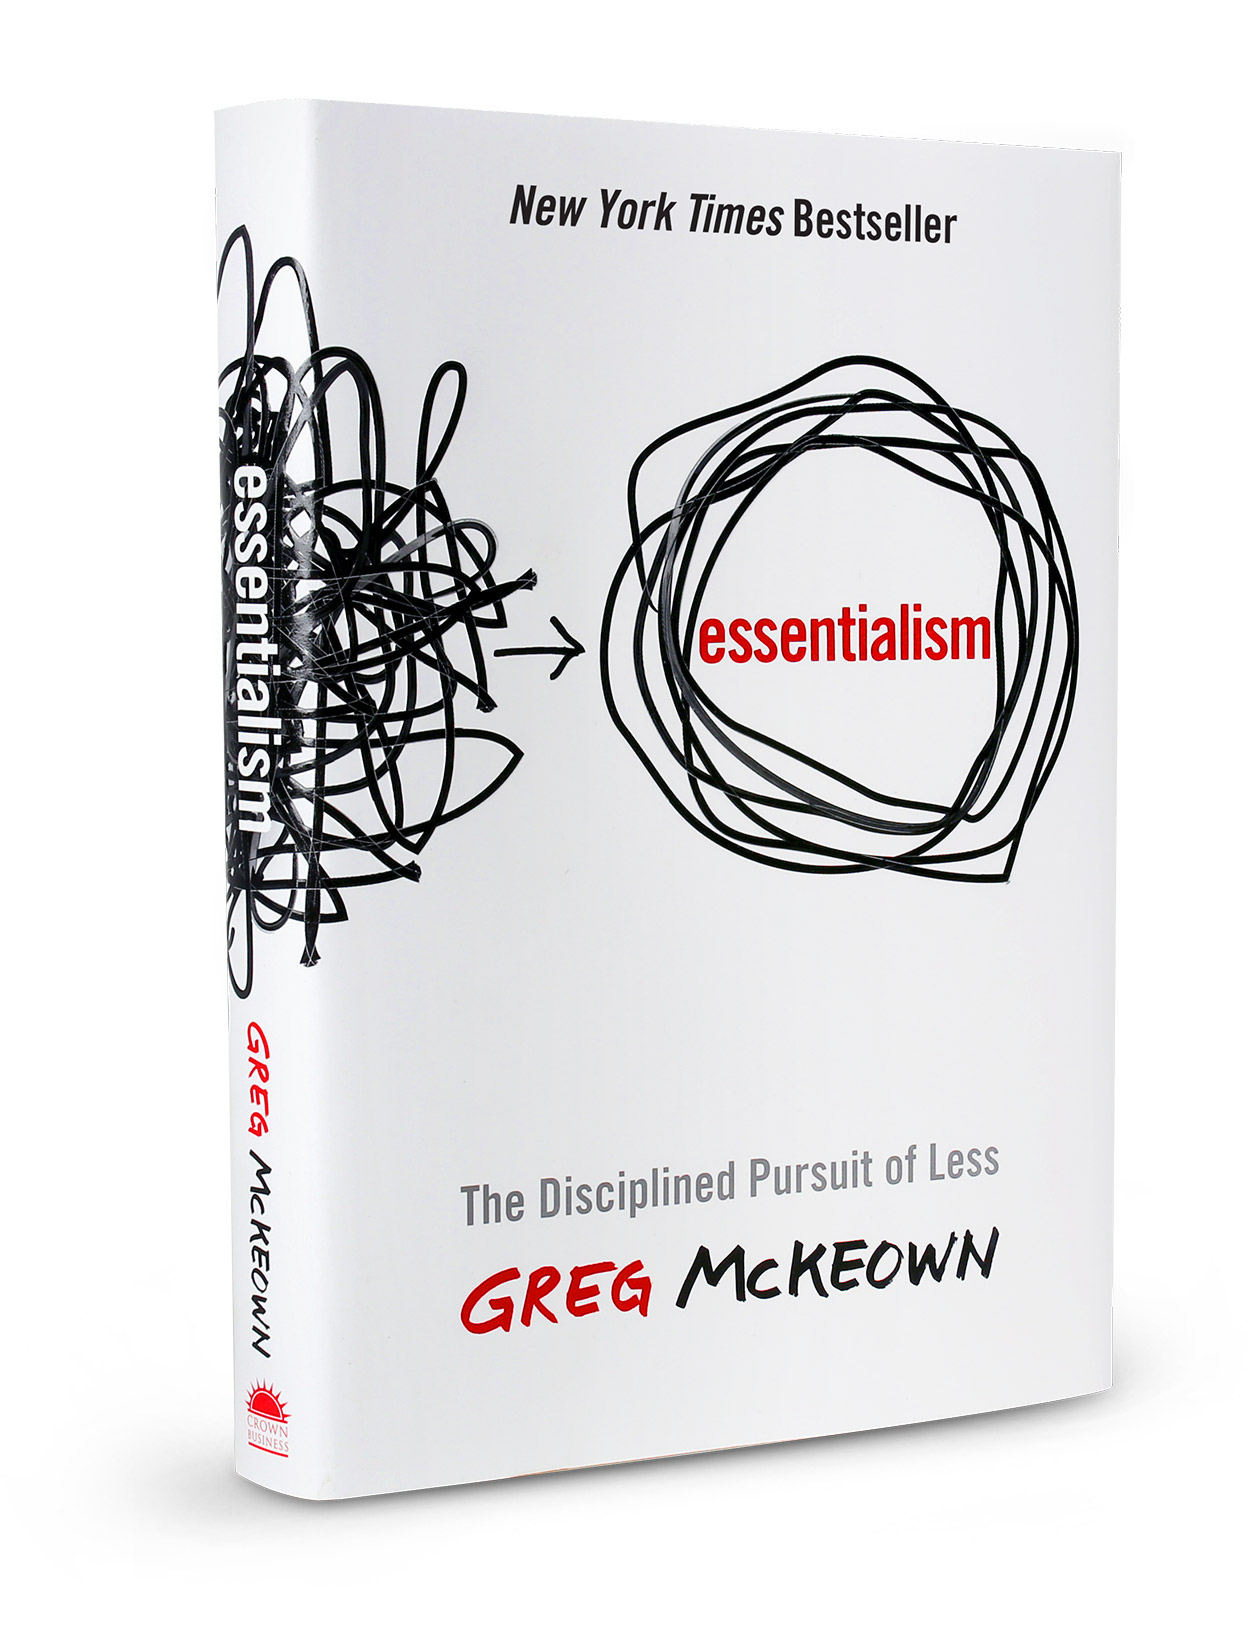
\includegraphics[width=\linewidth]{bookcover.jpg}

\heading{Overview}

\small

\icontext{Male}{12}{Greg McKeown}{black}\\[6pt]	
\icontext{Book}{12}{Essentialism: The Disciplined \\ Pursuit of Less}{black}\\[6pt]	
\icontext{MapMarker}{12}{NY}{black}\\[6pt]
\icontext{Calendar}{12}{2011}{black}\\[6pt]
\iconemail{Laptop}{12}{Book Website}{https://gregmckeown.com/book/}{black}\\[6pt]
\iconemail{Globe}{12}{Summary Source 1}{https://epigrammetry.hypotheses.org/595}{black}\\[6pt]
\iconemail{Globe}{12}{Summary Source 2}{https://epigrammetry.hypotheses.org/248}{black}\\[6pt]

\vspace{3em}

\begin{figure}[h]
    \centering
    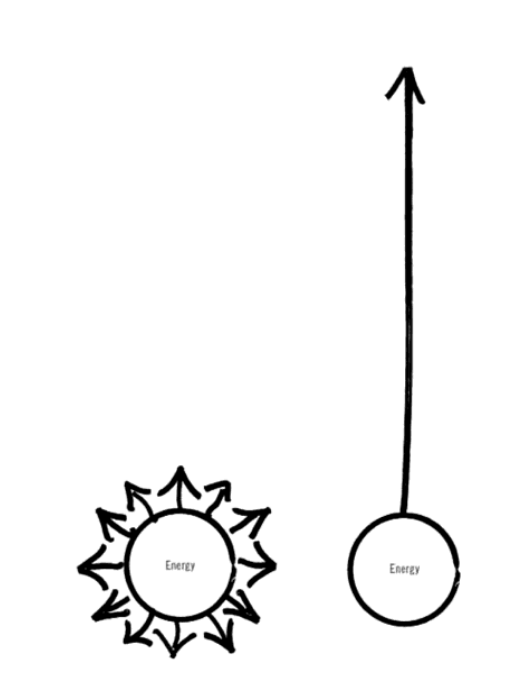
\includegraphics{essentialism-energy.png}
    \caption{Graph illustrating how far you can go with the same amount of energy if invested deliberately in just one thing versus diffusion}
    \label{fig:my_label}
\end{figure}


\normalsize
\switchcolumn

\titlebox{white}{darkcol}{

\bigfont{Essentialism} 

\titletext{Greg McKeown}

The Disciplined Pursuit of Less, NY 2011.
}
\vspace{1em}

%---------------------------------------------------------------------------------------


\heading{Summary}

The normal state of a closet is to get more and more cluttered if a conscious effort is not made to get rid of non-essentials. Consciously making this effort over and over again is what McKeown calls ‘disciplined’. 

\begin{quote}
    Essentialism is the disciplined pursuit of ‘less but better’.
\end{quote}

The clutter piles up again and every time it does, you need to act: You need to know where the next thrift store is and when it’s open. You need to have a plan in case somebody drops off their clutter in your closet.


\heading{Essentialist checklist}
\begin{itemize}
    \item Do less than you want to do / could do. 
    \item get enough sleep, drink enough water ('protect the asset')
    \item take time for 'serious play'
    \item If you don't know what’s important right now, what’s important right now is to find out what’s important right now. Only once you know this can you use your time effectively.
\end{itemize}

\heading{Actionable advice}
\begin{enumerate}
    \item 
    \textbf{Part two (“Explore”)} suggests you ‘escape’ and save time by being unavailable (ruthlessly avoid going to useless meetings, etc.); you see what really matters, make time for (serious) play, get enough sleep and select what you spend your time with using ‘extreme criteria’. 
    \item \textbf{Part III (“Eliminate”)} suggests you clarify decision making, dare to say no and learn how to do it gracefully without offending people, uncommit from non-essentials and gain freedom by setting boundaries for carefully ‘edited’ amount of meaningful activities.
    \item \textbf{Part IV (“Execute”)} praises using a “time buffer” between commitments, removing things which hurt your effectiveness most rather than starting some new quick fix technique on top of everything, progressing with small wins, using routine to get in the flow, focusing and being in the moment by asking (“What’s important now?”).
\end{enumerate}


\heading{Success spiral}

With clarity of purpose comes success. But with success come opportunities which distract you from your purpose and make you plateau. Now you have to subtract and say no politely. You only move forward if you put all your energy in the same direction. 


\heading{Essentialist mindset}
\begin{enumerate}
    \item There can only ever be one priority.
    \item Thus, trade-offs are real: you can either do this or that. By deciding on doing one thing, you discard the other. Make this an active choice.
    \item Remember the unimportance of practically everything: Say no and triage ruthlessly.
\end{enumerate}

You can't just fit it all in. Also, actions aren't all worth the same. Like in the Pareto principle (80/20), some actions have tremendously better effects than others which are practically useless in the pursuit of your goals. 



\end{paracol}
\end{document}

